\documentclass[brazilian, 12pt, a4paper, final]{article}
\usepackage[utf8]{inputenc}
\usepackage[brazil]{babel}
\usepackage[T1]{fontenc}
\usepackage{multicol}
\usepackage{graphicx}
\usepackage{indentfirst}
\usepackage{amsmath}
\usepackage{array}
\usepackage{caption}
\usepackage{float}
\usepackage{enumitem}
\usepackage[left=1.5cm, right=1.5cm]{geometry}

\title{\textbf{Método de Fehlberg na solução do problema de oscilações acopladas}}

\author{Cristiane de Paula Oliveira\\\\\small{Instituto de Física -- Universidade Federal do Rio Grande do Sul}}

\begin{document}

\maketitle

\begin{abstract}
  \noindent
  Nestre trabalho serão estudados blá blá blá. \\
  \\
  \textbf{Palavras-chave:} oscilações acopladas, método de Fehlberg, método de Runge-Kutta, solução numérica
\end{abstract}
\begin{multicols*}{2}
\section{Introdução}


\section{Formulação do problema}
Neste trabalho será estudado um sistema constituido por 4 osciladores acoplados executando oscilações longitudinais com os extremos fixos.

A energia cinética do sistema pode ser escrita como
\begin{equation}
	T=\frac{1}{2}m\sum_{i=1}^{4}\dot{\eta_i}^2
\end{equation}
e a energia potencial pode ser escrita como
\begin{equation}
	U=\frac{1}{2}k\eta_1^2+\frac{1}{2}k\sum_{i=1}^{3}(\eta_{i+1}-\eta_{i})^2 + \frac{1}{2}k\eta_4^2.
\end{equation}
 
 A lagrangiana $L=T-U$ desse sistema, portanto, é descrita por
 \begin{eqnarray}
 	 L=\frac{1}{2}m\sum_{i=1}^{4}\dot{\eta_i}^2-\frac{1}{2}k\eta_1^2-\frac{1}{2}k\sum_{i=1}^{3}(\eta_{i+1}-\eta_{i})^2 - \frac{1}{2}k\eta_4^2.
 \end{eqnarray}
 
 As equações do movimento de cada oscilador é dada pelas equações de Euler-Lagrange
 \begin{equation}
 	\frac{\partial L }{\partial\eta_i}-\frac{d}{dt}\frac{\partial L}{\partial \dot{\eta_i}}=0,\;\;\;\;\; (i=1,2,3,4).
 \end{equation}
Portanto, as equações acopladas são
\begin{eqnarray}
	\ddot{\eta_1}&=&\omega_0^2(\eta_2-2\eta_1), \\
	\ddot{\eta_2}&=&\omega_0^2(\eta_1-2\eta_2+\eta_3), \\
	\ddot{\eta_3}&=&\omega_0^2(\eta_2-2\eta_3+\eta_4), \\
	\ddot{\eta_4}&=&\omega_0^2(\eta_3-2\eta_4),
\end{eqnarray}
em que
\begin{equation}
	\omega_0^2=\frac{k}{m}.
\end{equation}

As soluções desse sistema de equações acopladas são
\begin{equation}
	\eta_j(t)=\sum_{r=1}^4\rho_{rj}[\mu_r \cos(\omega_r t)-\nu_r\sin(\omega_r t)],
\end{equation}
para $(j=1,2,3,4)$, em que
\begin{equation}
	\omega_r=2\omega_0\bigg\vert\sin\left(\frac{r\pi}{10}\right)\bigg\lvert
\end{equation}
são as autofrequências dos modos normais de oscilação,
\begin{equation}
	\rho_{rj}=\sqrt{\frac{2}{5}}\sin\left(\frac{rj\pi}{5}\right)
\end{equation}
são os autovetores associados às autofrequências dos modos normais de oscilações e $\mu_r$ e $\nu_r$ são aplitudes determinadas a partir das condições iniciais.

No problema analisado neste trabalho, as condições iniciais são
\begin{eqnarray}
	\eta_{j0}&=&\epsilon\delta_{j1} \\
	\dot{\eta_{j0}}&=&0,
\end{eqnarray}
para $(j=1,2,3,4)$.

\section{Métodos numéricos}

Os métodos numéricos que serão utilizados para resolver o sistema são descritos a seguir.

\subsection{Método de Runge-Kutta de 4ª ordem}
O método de Runge-Kutta de $4^{a}$ ordem consiste em encontrar
\begin{eqnarray}
 k_1&=&f(t_n;x_n)\,h, \\
 k_2&=&f\left(t_n+\frac{h}{2}; x_n +\frac{k_1}{2}\right)\,h, \\
 k_3&=&f\left(t_n+\frac{h}{2}; x_n +\frac{k_2}{2}\right)\,h \;\;\mathrm{ e} \\
 k_4&=&f\left(t_n+h; x_n + k_3\right)\,h,
\end{eqnarray}
\noindent
de forma que
\begin{equation}
 x_{n+1}=x_{n}+\frac{1}{6}\left(k_1+2\,k_2+2\,k_3+k_4\right). 
\end{equation}
\noindent
onde $f(t,x)=\frac{dx}{dt}$ e $h$ é o tamanho do passo.

\subsection{Método de Fehlberg}
Este método utiliza um método de Runge-Kutta com erro de truncamento local de ordem 5 para obter uma estimativa do erro local num método de Runge-Kutta de ordem 4.

O método de Runge-Kutta de ordem 5 é
\begin{equation}
  x_{n+1}=x_n+c_1k_1+c_2k_2+c_3k_3+c_4k_4+c_5k_5+c_6k_6,
\end{equation}
e o  método de Runge-Kutta de ordem 4 é
\begin{equation}
  x_{n+1}^*=x_n^*+c_1^*k_1+c_2^*k_2+c_3^*k_3+c_4^*k_4+c_5^*k_5+c_6^*k_6,
\end{equation}
onde
\begin{eqnarray}
  k_1&=&f(t_n;x_n)\,h,\\
  k_2&=&f(t_n +a_2h;x_n+b_{21}k_1)\,h,\\
  k_3&=&f(t_n +a_3h;x_n+b_{31}k_1+b_{32}k_2)\,h,\\
  \nonumber & & \dots \\
  k_6&=&f(t_n+a_6h;x_n+b_{61}k_1+b_{62}k_2+\nonumber \\
     & &b_{63}k_3+b_{64}k_4+b_{65}k_5)\,h. 
\end{eqnarray}

Os coeficientes $c_i$,$c_i^*$ e $a_i$,(i=1,2,...,6), e os coeficientes $b_{i,j}$,(i,j=1,2,...,6) e (i>j), são encontradas tabeladas.

A estimativa do erro corrente $\epsilon_c$ é
\begin{equation}
  \epsilon_c=|x_{n+1}-x_{n+1}^*|.
\end{equation}

A partir dessa estimativa do erro,
se $\epsilon_c \le \epsilon$, utiliza-se esse passo e calcula-se um novo $h$ pela equação (\ref{eq:novo_h}) para o passo seguinte. Se $\epsilon_c > \epsilon$, rejeita-se esse $h$ e calcula-se um novo passo pela equação (\ref{eq:novo_h}) para esse mesmo ponto.

\begin{equation}\label{eq:novo_h}
  h_{novo}=h\left(\frac{\epsilon}{2\epsilon_c}\right)^{\frac{1}{4}},
\end{equation}
em que $\epsilon$ é a tolerância do erro.

\section{Resultados e análises}


\begin{figure}[H] 
  \centering
  %\includegraphics[width=0.34\textwidth,angle=-90]{mapa_a120_b250.eps}
  \caption{Mapa para $a=1,2$ e $b=2,5$.}
  \label{fig:120}
\end{figure}


\section{Considerações finais}
 
\begin{thebibliography}{n}
\bibitem{Marotto}  F. R. ~Marotto. {\em Snap-Back Repellers Imply Chaos in ${\rm I\!R}^{n}$}, Journal of Mathematical Analysis and Aplications {\bf 63}, 199-223 (1978)
 
\bibitem{Paper} S. M. ~Salman, A. A. ~Elsadany. {\em On the bifurcation of Marotto’s map and its application in image encryption}, Journal of Computational and Applied Mathematics {\bf 328}, 177–196 (2018)

\bibitem{Book} L. H. A, ~Monteiro. {\em Sistemas Dinâmicos}, (editora Livraria da Física, 3ª edição, 2011)
  
\end{thebibliography}
\end{multicols*}

\appendix
\section{APÊNDICE - INSTRUÇÕES}

Para compilar e rodar todos os programas utiliza-se o script:
\begin{verbatim}
$ sh Coupled.sh
\end{verbatim}

Ao final, plota-se os gráficos utilizando:
\begin{verbatim}
gnuplot> load 'PlotAll.gnu'
\end{verbatim}

\end{document}
